\documentclass[10pt,letterpaper,bibliography=totoc]{scrartcl}

\usepackage[letterpaper,margin=1.2in]{geometry}
\usepackage{helvet}
\usepackage[utf8]{inputenc}
\usepackage{graphicx}
\usepackage[hyphens]{url}
\usepackage{hyperref}
\usepackage[all]{hypcap} 
\usepackage{xcolor}
\usepackage{listings}
\usepackage[T1]{fontenc}
\usepackage{verbatim}
\usepackage[parfill]{parskip}

\lstset{
    basicstyle=\scriptsize,
    numbers=left,
    numberstyle=\scriptsize,
    stepnumber=1,
    numbersep=5pt,
    showspaces=false,
    showstringspaces=false,
    showtabs=false,
    frame=shadowbox,
    tabsize=4,
    captionpos=b,
    breaklines=true,
    breakatwhitespace=false,
    keywordstyle=\color{blue!70},
    commentstyle=\color{red!50!green!50!blue!50},
    rulesepcolor=\color{red!20!green!20!blue!20},
    numberbychapter=false,
    stringstyle=\ttfamily
}

\setcounter{tocdepth}{2}

\hypersetup{
    colorlinks=true,
    breaklinks=true,
    urlcolor=blue,
    linkcolor=black
}

\begin{document}

\author{Orkun Krand}
\title{Assignment 4}
\subtitle{Fall 2017\\ CS834 Introduction to Information Retrieval\\ Dr. Michael Nelson}
\maketitle
\newpage

\section{Question 8.3}
\subsection {Question}
For one query in the CACM collection (provided at the book website), generate a ranking using Galago, and then calculate average precision, NDCG at 5 and 10, precision at 10, and the reciprocal rank by hand.

\subsection{Methodology}
Using \href{https://sourceforge.net/p/lemur/wiki/Galago/}{Galago}, I was able to create an index of the \href{http://www.search-engines-book.com/collections/}{CACM corpus}. Afterwards, I used Galago to search for the queries. I used \texttt{galago.py} to issue the queries and find the required values. I utilized \href{http://docs.python-requests.org/en/master/}{Requests} and \href{https://www.crummy.com/software/BeautifulSoup/}{Beautiful Soup} to issue the queries and parse the results. 

Precision is the true positive divided by the total positive (true and false) while recall is true positive divided by true positive and false negative. In order to get the precision at specific rankings, I had to calculate cumulative precision at each rank. For the average precision, I computed the sum of precisions at each rank for the retrieved relevant documents and then divided this sum by the same set. NDCG was calculated by dividing DCG by IDCG. The two values were computed using the formulas in the textbook\cite{classtext}. Reciprocal rank is 1 divided by the rank of the first relevant document. 

\subsection{Results}
Using query 13 (code optimization for space efficiency), I got the following results:
\begin{figure}[h!]
\centering
\label{fig:q13}
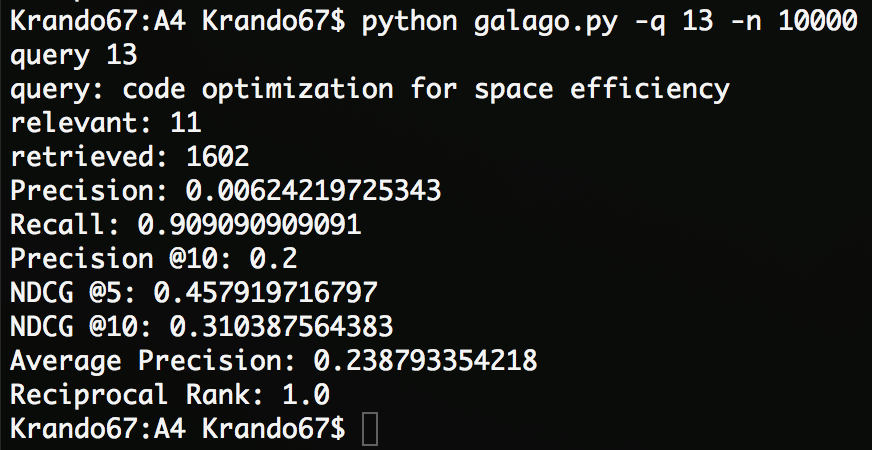
\includegraphics[scale=.5]{query13.png}
\caption{Query 13 Results}
\end{figure}

\section{Question 8.4}
\subsection {Question}
For two queries in the CACM collection, generate two uninterpolated recall-precision graphs, a table of interpolated precision values at standard recall levels, and the average interpolated recall-precision graph.

\subsection{Methodology}
Deciding to go with queries 9 and 10, the following graphs were created using \texttt{graph.R} and the table was created using \texttt{ipr.py}. In order to minimize clutter, I joined the two uninterpolated recall-precision graphs into one graph, distinguished by color.

\subsection{Results}
\begin{figure}[h!]
\centering
\label{fig:unint910}
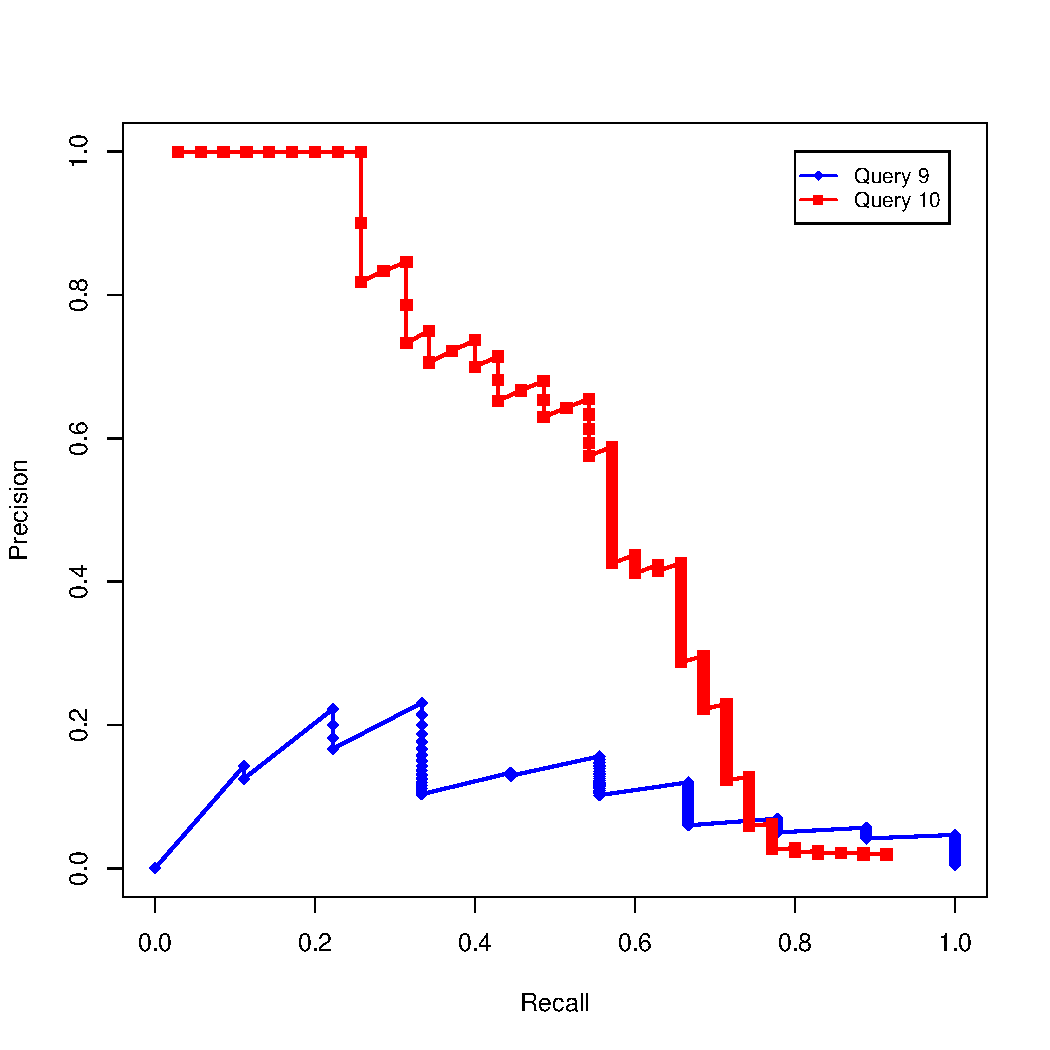
\includegraphics[scale=.5]{unint910.pdf}
\caption{Uninterpolated recall-precision graphs for queries 9 and 10}
\end{figure}

\begin{table}[h!]
\centering
\begin{tabular}{ l l l l l l l l l l l l }
Recall & 0.0 & 0.1 & 0.2 & 0.3 & 0.4 & 0.5 & 0.6 & 0.7 & 0.8 & 0.9 & 1.0 \\
\cline{2-12}
Query 9 & 0.231 & 0.231 & 0.231 & 0.231 & 0.156 & 0.156 & 0.12 & 0.0693 & 0.0567 & 0.0466 & 0.0466 \\
\cline{2-12}
Query 10 & 1 & 1 & 1 & 0.846 & 0.714 & 0.655 & 0.426 & 0.229 & 0.0237 & 0.0198 & 0.0198 \\
\cline{2-12}
Average & 0.615 & 0.615 & 0.615 & 0.538 & 0.435 & 0.406 & 0.273 & 0.149 & 0.0402 & 0.0332 & 0.0332 \\
\cline{2-12}
\end{tabular}
\caption{Interpolated precision values at standard recall levels}
\label{tab:ipr}
\end{table}

\begin{figure}[h!]
\centering
\label{fig:int910}
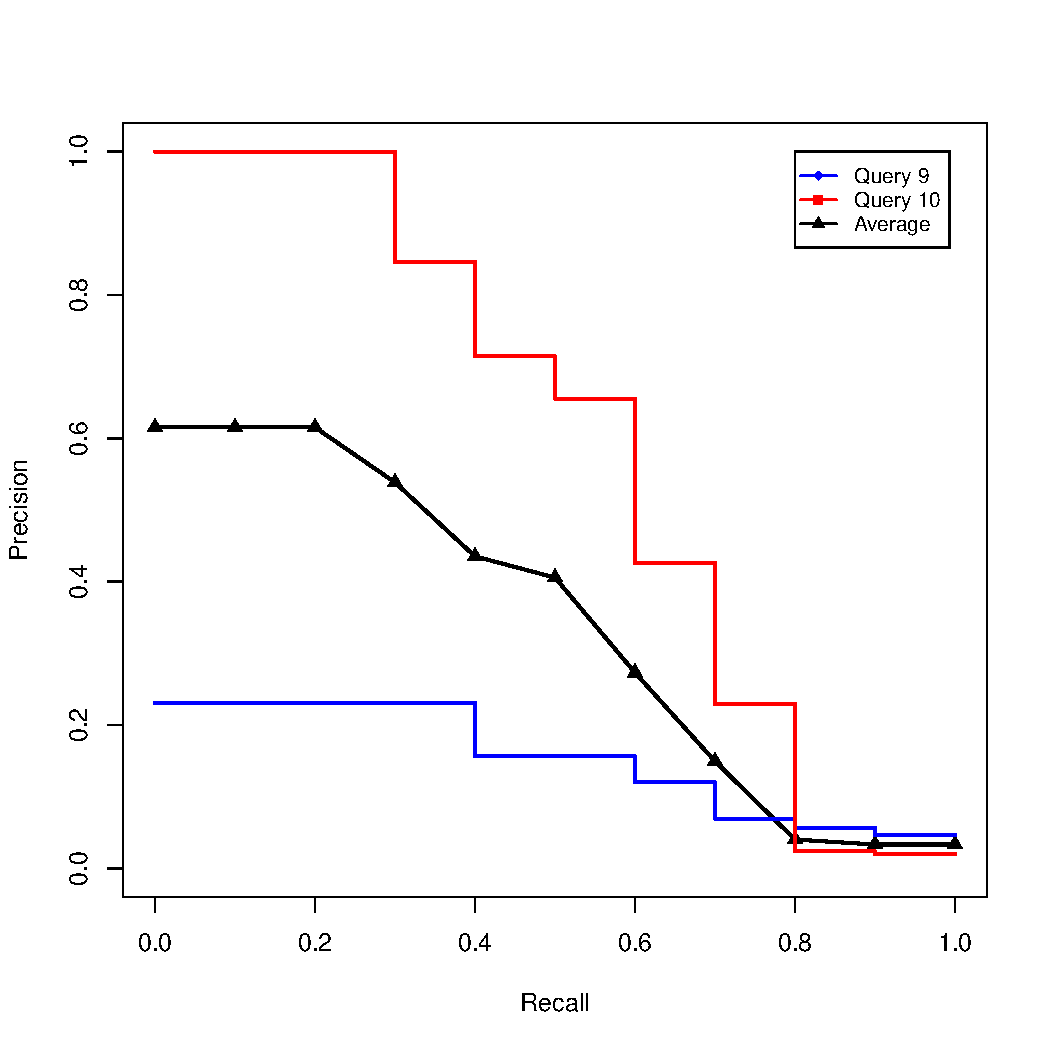
\includegraphics[scale=.5]{int910.pdf}
\caption{Average interpolated recall-precision graphs for queries 9 and 10}
\end{figure}

\section{Question 8.5}
\subsection{Question}
Generate the mean average precision, recall-precision graph, average NDCG at 5 and 10, and precision at 10 for the entire CACM query set.

\subsection{Methodology}
\texttt{entirecacm.py} was created to calculate the values for the entire query set. \texttt{graph.R} was modified to produce the requested recall-precision graph. 

\subsection{Results}
\begin{figure}[h!]
\centering
\label{fig:cacm}
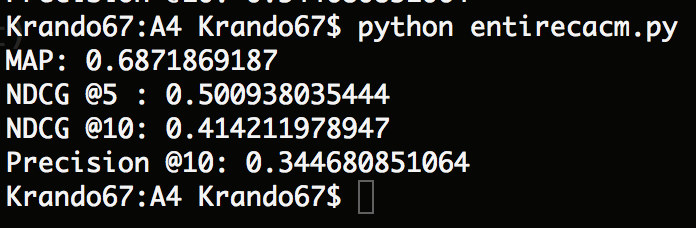
\includegraphics[scale=.5]{entirecacm.png}
\caption{Entire CACM Results}
\end{figure}
\begin{figure}[h!]
\centering
\label{fig:overallavg}
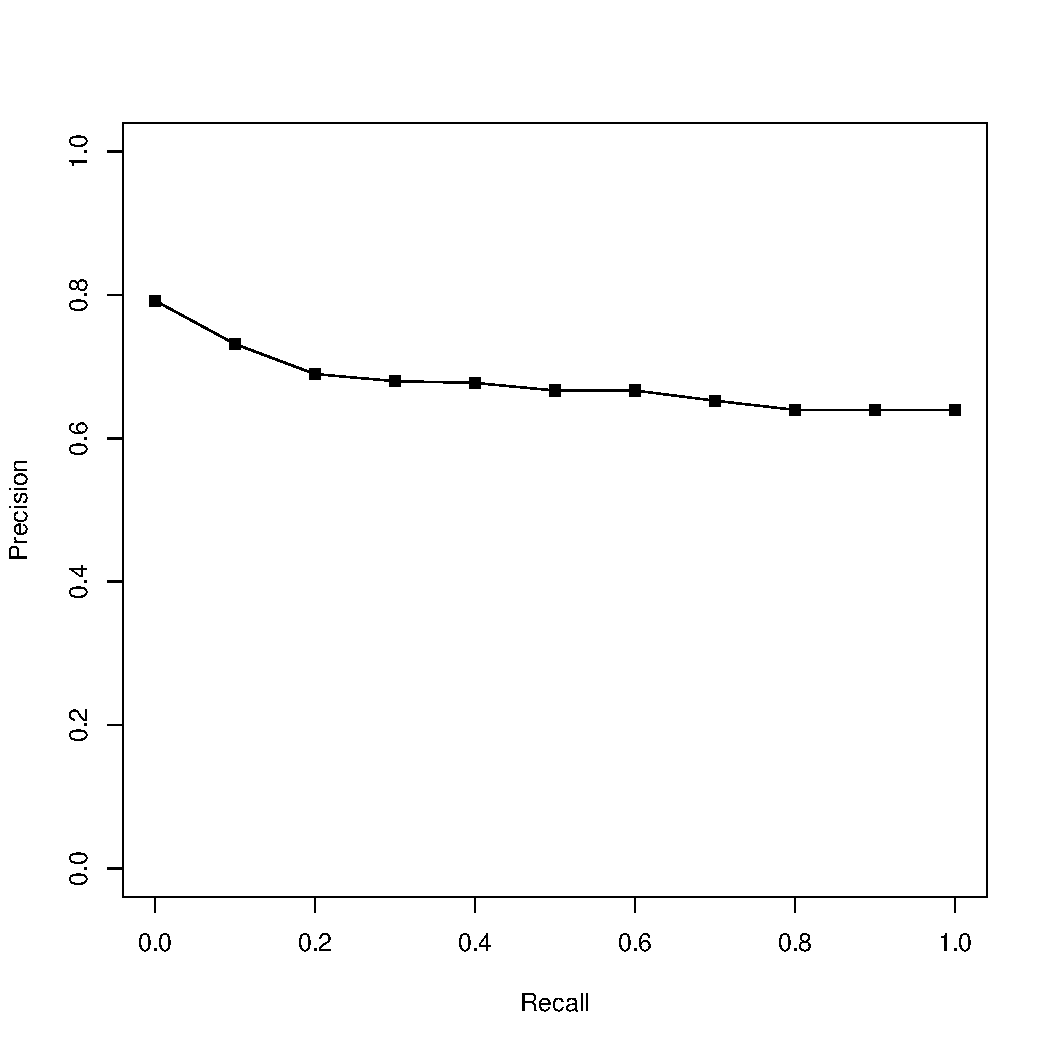
\includegraphics[scale=.5]{avgall.pdf}
\caption{CACM queries recall-precision graph}
\end{figure}

\section{Question 8.7}
\subsection {Question}
Another measure that has been used in a number of evaluations is R-precision.  This is defined as the precision at R documents, where R is the number of relevant documents for a query. It is used in situations where there is a large variation in the number of relevant documents per query. Calculate the average \textit{R-precision} for the CACM query set and compare it to the other measures.

\subsection{Methodology}
Using \texttt{Rprecision.py}, which was run over all documents, I was able to get the R precision at any query I want. Other measures were displayed along with the result for easy comparison. 

\subsection{Results}
\begin{figure}[h!]
\centering
\label{fig:rprecision}
\includegraphics[scale=.5]{rprecision.png}
\caption{R precision for query 17}
\end{figure}

At all queries I tried, I observed that R-precision value is very close to the average precision. So it seems that it's a good candidate for an alternative. However, it may not be as stable with a small set of relevant documents. 

\section{Question 8.9}
\subsection{Question}
For one query in the CACM collection, generate a ranking and calculate BPREF. Show that the two formulations of BPREF give the same value.

\subsection{Methodology}
Two functions which calculate the two equations for BPREF found in the textbook\cite{classtext} were added to \texttt{galago.py}.

\subsection{Results}
After spending time writing the code for BPREF which can be found in \texttt{bpref.py}, I had to run it at least 3 times. The results are below. While the two BPREF values weren't exactly the same they were very close.

\begin{figure}[h!]
\centering
\label{fig:bpref}
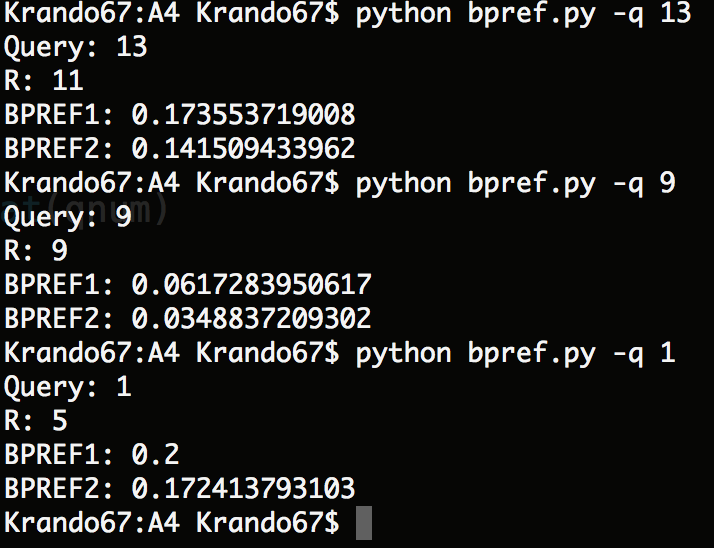
\includegraphics[scale=.5]{bpref.png}
\caption{BPREF values for multiple queries}
\end{figure}

\clearpage
\begin{thebibliography}{9}
\bibitem{classtext}
    Croft, William Bruce, et al. \textit{Search Engines: Information Retrieval in Practice}. Pearson, 2010.
\end{thebibliography}
\end{document}